%\documentclass{article}
\documentclass[article,shortnames,nojss]{jss}
\usepackage{amssymb}
\usepackage{natbib}
\usepackage{graphicx}
\usepackage{color}
\usepackage{verbatim}
\usepackage{hyperref}
\usepackage{url}
%\usepackage{ae}



\setlength{\unitlength}{1cm}
\newcommand{\ex}[1]{\ensuremath{\mathbb{E}[#1]}}
\newcommand{\var}[1]{\ensuremath{\mathrm{Var}[#1]}}
\newcommand{\cov}[1]{\ensuremath{\mathrm{Cov}[#1]}}
\newcommand{\corr}[1]{\ensuremath{\mathrm{Corr}[#1]}}
\newcommand{\bd}[1]{\ensuremath{\mbox{\boldmath $#1$}}}

%\VignetteIndexEntry{Vignette for CARBayes  package.}


%% almost as usual
\author{Duncan Lee\\University of Glasgow }
\title{\pkg{CARBayes} version 5.2: An \proglang{R} Package for Spatial Areal Unit Modelling  with Conditional Autoregressive Priors}

%% for pretty printing and a nice hypersummary also set:
\Plainauthor{Duncan Lee} %% comma-separated
\Plaintitle{CARBayes version 5.2: An R package for spatial areal unit modelling  with conditional autoregressive priors} %% without formatting
\Shorttitle{\pkg{CARBayes}: Bayesian Conditional Autoregressive modelling} %% a short title (if necessary)

%% an abstract and keywords
\Abstract{
This is a vignette for the \proglang{R} package \pkg{CARBayes} version 5.2, and is an updated version of a paper in the Journal of Statistical Software in 2013 Volume 55 Issue 13 by the same author. The package implements univariate and multivariate spatial generalised linear mixed models for areal unit data, with inference in a Bayesian setting using Markov chain Monte Carlo (MCMC) simulation. The response variable can be binomial, Gaussian, multinomial, Poisson or zero-inflated Poisson (ZIP), and spatial autocorrelation is modelled by  a set of random effects that are assigned a conditional autoregressive (CAR) prior distribution. A number of different models are available for univariate spatial data, including models with no random effects as well as random effects modelled by different types of CAR prior. Additionally, a multivariate CAR (MCAR) model for multivariate spatial data is available, as is a two-level hierarchical model for modelling data relating to individuals within areas. The initial creation of this package was supported by the Economic and Social Research Council (ESRC) grant RES-000-22-4256, and on-going development has been supported by the Engineering and Physical Science Research Council (EPSRC) grant EP/J017442/1, ESRC grant ES/K006460/1, Innovate UK / Natural Environment Research Council (NERC) grant NE/N007352/1, and the TB Alliance. 
}

\Keywords{Bayesian inference, conditional autoregressive priors, \proglang{R} package \pkg{CARBayes}}
\Plainkeywords{Bayesian inference, conditional autoregressive priors, R package CARBayes}



\Address{
  Duncan Lee\\
  School of Mathematics and Statistics\\ 
  University Place\\  
  University of Glasgow\\
  Glasgow\\ 
  G12 8SQ, Scotland\\
  E-mail: \email{Duncan.Lee@glasgow.ac.uk}\\
  URL: \url{http://www.gla.ac.uk/schools/mathematicsstatistics/staff/duncanlee/}
}
%% The address of (at least) one author should be given
%% in the following format:

\usepackage{Sweave}
\begin{document}
\Sconcordance{concordance:CARBayes.tex:CARBayes.Rnw:%
1 55 1 1 0 6 1 1 4 336 1 1 2 1 0 5 1 3 0 1 2 2 1 1 2 1 0 2 1 3 0 1 2 11 %
1 1 2 1 0 4 1 12 0 1 2 21 1 1 2 1 0 1 1 3 0 1 2 3 1 1 2 1 0 1 1 3 0 1 2 %
10 1 1 2 4 0 1 2 5 1 1 2 1 0 1 2 4 0 1 2 2 1 1 2 1 0 1 1 1 7 6 0 1 1 3 %
0 1 2 13 1 1 2 1 0 2 1 28 0 1 2 2 1 1 2 1 0 3 1 13 0 1 2 7 1 1 2 4 0 1 %
2 179 1 1 2 1 0 4 1 12 0 1 2 3 1 1 2 4 0 1 2 2 1 1 3 5 0 1 2 4 1 1 2 1 %
0 1 1 1 7 6 0 1 1 3 0 1 2 12 1 1 2 1 0 1 1 3 0 1 2 12 1 1 2 1 0 1 1 3 0 %
1 2 97 1}


%%%%%%%%%%%%%%
%%%% Section 1
%%%%%%%%%%%%%%




\section{Introduction}
Data relating to a set of non-overlapping spatial areal units are prevalent in many fields, including agriculture (\cite{besag1999}), ecology (\cite{brewer2007}), education (\cite{wall2004}), epidemiology (\cite{lee2011}) and image analysis (\cite{gavin1997}).  There are numerous motivations for modelling such data, including ecological regression  (see \cite{wakefield2007} and \cite{lee2009}), disease mapping (see \cite{green2002} and \cite{lee2011}) and Wombling (see \cite{lu2007}, \cite{ma2007}). The set of areal units on which data are recorded can form a regular lattice or differ largely in both shape and size, with examples of the latter including the set of electoral wards or census tracts corresponding to a city or country. In either case such data typically exhibit spatial autocorrelation, with observations from areal units close together tending to have similar values. A proportion of this spatial autocorrelation may be modelled by known covariate risk factors in a regression model, but it is common for  spatial structure to remain in the residuals after accounting for these covariate effects. This residual spatial autocorrelation can be induced by unmeasured confounding, neighbourhood effects, and grouping effects.

\hspace{1cm} The most common remedy for this residual autocorrelation is to augment the linear predictor with a set of spatially autocorrelated random effects, as part of a Bayesian hierarchical model. These random effects are typically represented with a conditional autoregressive (CAR, \cite{besag1991}) prior,  which induces spatial autocorrelation through the adjacency structure of the areal units. A number of CAR priors have been proposed in the literature, including the intrinsic and Besag-York-Molli\'{e} (BYM) models (both \cite{besag1991}), as well as the alternative  developed by \cite{leroux2000}. 

\hspace{1cm} However, these CAR priors force the random effects to exhibit a single global level of spatial autocorrelation, ranging from independence through to strong spatial smoothness. Such a uniform level of spatial autocorrelation for the entire region maybe unrealistic for real data, which instead may exhibit sub-regions of spatial autocorrelation separated by discontinuities. A number of approaches have been proposed for extending the class of CAR priors to deal with localised spatial smoothing amongst the random effects, including \cite{lee2012}, and \cite{lee2015}.

\hspace{1cm} The models described above are typically implemented in a Bayesian setting, where inference is based on Markov chain Monte Carlo (MCMC) simulation. The most commonly used software to implement this class of models is the \proglang{BUGS} project (\cite{lunn2009}, \proglang{WinBUGS} and \proglang{OpenBUGS}), which has in-built functions to implement the intrinsic and BYM models. CAR models can also be implemented in \proglang{R} using Integrated Nested Laplace Approximations (INLA, \emph{http://www.r-inla.org/}), using the package \pkg{INLA} (\citealp{rue2009}).

\hspace{1cm} \pkg{CARBayes} (\citealp{lee2013}) is the premier \proglang(R) package for modelling spatial areal unit data with conditional autoregressive type spatial autocorrelation structures in a Bayesian setting using MCMC simulation. Its main advantages are firstly ease of use because: (1) the spatial adjacency information is easy to specify as a neighbourhood (adjacency) matrix; and (2) given the neighbourhood matrix, models can be implemented by a single function call. Secondly, \pkg{CARBayes} can implement a much wider class of spatial areal unit models than say \proglang{WinBUGS}, and the univariate or multivariate response data can follow binomial, Gaussian, multinomial, Poisson or zero-inflated Poisson (ZIP) distributions, while a range of CAR priors can be specified for the random effects. Additionally, a two-level hierarchical model is available for modelling data relating to individuals within areas. Spatio-temporal models for areal unit data using CAR type priors can be implemented using the sister package \pkg{CARBayesST} (\citealp{carbayesst}).

\hspace{1cm} The aim of this vignette is to present \pkg{CARBayes}, by outlining the class of models that it can implement and illustrating its use by means of 3 worked examples. Section 2 outlines the general Bayesian hierarchical model that can be implemented in the \pkg{CARBayes} package, while Section 3 details the inputs and outputs for the software.  Sections 4 to 6 give three worked examples of using the software, including how to create the neighbourhood matrix and produce spatial maps of the results. Finally, Section 7 contains a concluding discussion, and outlines areas for future development.


%%%%%%%%%%%%%%
%%%% Section 2
%%%%%%%%%%%%%%
\section{Spatial models for areal unit data}
This section outlines the class of spatial generalised linear mixed models for areal unit data that can be implemented in \pkg{CARBayes}. Inference for all models is set in a Bayesian framework using MCMC simulation. The majority of the models in \pkg{CARBayes} relate to univariate spatial data and are described in Section 2.1, while models for multivariate spatial data and two-level data relating to individuals within areas are described in Sections 2.2 and 2.3.


\subsection{Univariate spatial data models}
The study region $\mathcal{S}$ is partitioned into $K$ non-overlapping areal units $\mathcal{S}=\{\mathcal{S}_{1},\ldots,\mathcal{S}_{K}\}$, which are linked to a corresponding set of responses $\mathbf{Y}=(Y_{1},\ldots,Y_{K})$, and a vector of known offsets $\mathbf{O}=(O_{1},\ldots,O_{K})$. Missing, \code{NA}, values are allowed in the response $\mathbf{Y}$ except for the \code{S.CARlocalised()} function, which does not allow them due to model complexity and corresponding poor predictive performance. These missing values are treated as additional unknown parameters, and are updated in the MCMC algorithm using a data augmentation approach \cite{tanner1987}. The spatial variation in the response is modelled by a matrix of covariates $\mathbf{X}=(\mathbf{x}_{1},\ldots,\mathbf{x}_{K})$ and  a spatial structure component $\bd{\psi}=(\psi_{1},\ldots,\psi_{K})$, the latter of which is included to model any spatial autocorrelation that remains in the data after the covariate effects have been accounted for. The vector of covariates for areal unit $\mathcal{S}_{k}$ are denoted by $\mathbf{x}_{k}=(1, x_{k1},\ldots,x_{kp})$, the first of which corresponds to an intercept term. The general spatial generalised linear mixed model is given by


\begin{eqnarray}
Y_{k}|\mu_{k}&\sim&f(y_{k}|\mu_{k},\nu^{2})~~~~\mbox{for }k=1,\ldots,K\label{equation likelihood}\\
g(\mu_{k})&=& \mathbf{x}_{k}^{\top}\bd{\beta} + O_k + \psi_{k}\nonumber\\
\bd{\beta}&\sim&\mbox{N}(\bd{\mu}_{\beta} \bd{\Sigma}_{\beta})\nonumber\\
\nu^2 &\sim& \mbox{Inverse-Gamma}(a,b).\nonumber
\end{eqnarray}

The expected value of $Y_{k}$ is denoted by $\E(Y_{k})=\mu_{k}$, while $\nu^{2}$ is an additional scale parameter that is required if the Gaussian family is used. The latter is assigned a conjugate inverse-gamma prior distribution,  where the default specification is $\nu^{2}\sim\mbox{Inverse-Gamma}(1, 0.01)$. The vector of regression parameters are denoted by $\bd{\beta}=(\beta_{1},\ldots,\beta_{p})$, and non-linear covariate effects can be incorporated into the above model by including natural cubic spline or polynomial basis functions of the covariates in $\mathbf{X}$. A multivariate Gaussian prior is assumed for $\bd{\beta}$, and the mean $\bd{\mu}_{\beta}$ and diagonal variance matrix $\bd{\Sigma}_{\beta}$ can be chosen by the user. Default values specified by the software are a constant zero-mean vector and diagonal elements of  $\bd{\Sigma}_{\beta}$ equal to 100,000. The expected values of the responses are related to the linear predictor via an invertible link function $g(.)$, and \pkg{CARBayes} can fit the following data likelihood models:

\begin{itemize}
\item \textbf{Binomial - } $Y_{k}~\sim~\mbox{Binomial}(n_{k}, \theta_{k})$ and $\ln(\theta_{k}/(1-\theta_{k}))~=~\mathbf{x}_{k}^{\top}\bd{\beta} + O_{k} + \psi_{k}$. 

\item \textbf{Gaussian - } $Y_{k}~\sim~\mbox{N}(\mu_{k}, \nu^{2})$ and $\mu_{k}~=~\mathbf{x}_{k}^{\top}\bd{\beta} + O_{k} + \psi_{k}$. 

\item \textbf{Poisson - } $Y_{k}~\sim~\mbox{Poisson}(\mu_{k})$ and $\ln(\mu_{k})~=~\mathbf{x}_{k}^{\top}\bd{\beta} + O_{k} + \psi_{k}$. 

\item \textbf{ZIP - } $Y_{k}~\sim~\mbox{ZIP}(\mu_{k}, \omega_k)$. The zero-inflated Poisson model is used to represent data containing an excess of zeros, and is a mixture of a point mass distribution based at zero and a Poisson distribution with mean $\mu_{k}$. The probability that observation $Y_k$ is in the point mass distribution based at zero (called a structural zero) is $\omega_k$, and $(\mu_k, \omega_k)$ are modelled by

$$\ln(\mu_{k})~=~\mathbf{x}_{k}^{\top}\bd{\beta} + O_{k} + \psi_{k}\hspace{1cm}
\ln\left(\frac{\omega_k}{1-\omega_k}\right)~=~\mathbf{v}_{k}^{\top}\bd{\delta} + O^{(2)}_{k}.$$

Here $(\mathbf{v}_{k}, O^{(2)}_{k})$ are respectively covariates and an offset term that determine the probability that observation $Y_k$ is in the point mass distribution, while $\bd{\delta}$ are the corresponding regression parameters. In implementing the model a binary random variable $Z_k$ is sampled for each observation $Y_k$, where $Z_k=1$ if $Y_k$ comes from the point mass distribution, and $Z_k=0$ if $Y_k$ comes from the Poisson distribution. Further details about ZIP models are given by \cite{ugarte2004}.
\end{itemize}

In the binomial model above $n_k$ is the number of trials in the $k$th area, while $\theta_k$ is the probability of success in a single trial.   \pkg{CARBayes} can implement a number of different spatial random effects models for $\bd{\psi}$, and they are summarised below.


\begin{itemize}
\item \code{S.glm()} - fits a model with no random effects and thus is a generalised linear model. This model can be implemented with binomial, Gaussian, Poisson and ZIP data likelihoods.

\item \code{S.CARbym()} - fits the convolution or Besag-York-Mollie (BYM) CAR model outlined in \cite{besag1991}. This model can be implemented with binomial, Poisson and zip data likelihoods.

\item \code{S.CARleroux()} - fits the CAR model proposed by \cite{leroux2000}. This model can also fit the intrinsic CAR model proposed by \cite{besag1991}, as well as a model with independent random effects. This model can be implemented with binomial, Gaussian, Poisson and ZIP data likelihoods.

\item \code{S.CARdissimilarity()} - fits the localised spatial autocorrelation model proposed by \cite{lee2012}. This model can be implemented with binomial, Gaussian and Poisson data likelihoods.

\item \code{S.CARlocalised()} - fits the localised spatial autocorrelation model proposed by \cite{lee2015}. This model can be implemented with binomial and Poisson data likelihoods.
\end{itemize}


The spatial structure component $\bd{\psi}$ includes a set of random effects $\bd{\phi}=(\phi_{1},\ldots,\phi_{K})$, which come from a conditional autoregressive model. These models can be written in the general form $\bd{\phi}\sim\mbox{N}(\mathbf{0},\tau^{2}\mathbf{Q}(\mathbf{W})^{-1})$, where $\mathbf{Q}(\mathbf{W})$ is the precision matrix that may be singular (intrinsic model). This matrix controls the spatial autocorrelation structure of the random effects, and is based on a non-negative symmetric $K\times K$ neighbourhood (or adjacency) matrix $\mathbf{W}$. The kj$th$ element of the neighbourhood matrix $w_{kj}$ represents the spatial closeness between areas $(\mathcal{S}_k, \mathcal{S}_j)$, with positive values denoting geographical closeness and zero values denoting non-closeness. Additionally, diagonal elements $w_{kk}=0$.

\hspace{1cm} A binary specification for  $\mathbf{W}$ based on geographical contiguity is most commonly used, where $w_{kj}=1$ if areal units $(\mathcal{S}_k, \mathcal{S}_j)$ share a common border (denoted $k\sim j$), and is zero otherwise. This specification forces $(\phi_k, \phi_j)$ relating to geographically adjacent areas (that is where $w_{kj}=1$) to be autocorrelated, whereas random effects relating to non-contiguous areal units (that is where $w_{kj}=0$) are conditionally independent given the values of the remaining random effects. A binary specification is not necessary in \pkg{CARBayes} except for the function \code{S.CARdissimilarity()}, as the only requirement is that $\mathbf{W}$ is non-negative and symmetric. However, each area must have at least one positive element $\{w_{kj}\}$, meaning the row sums of $\mathbf{W}$  must be positive. CAR priors are commonly specified as a set of $K$ univariate full conditional distributions $f(\phi_{k}|\bd{\phi}_{-k})$ for $k=1,\ldots,K$, where $\bd{\phi}_{-k}=(\phi_{1},\ldots,\phi_{k-1},\phi_{k+1},\ldots,\phi_{K})$, which is how they are presented below. We now outline the five models that \pkg{CARBayes} can fit.\\

\subsubsection{A model with no random effects}
\code{S.glm()}\\
The simplest model that \pkg{CARBayes} can implement is a generalised linear model, which is based on (\ref{equation likelihood}) with the simplification that $\psi_k=0$ for all areas $k$. 

\subsubsection{Globally smooth CAR models}
\code{S.CARbym()}\\
The  convolution or Besag-York-Mollie (BYM) CAR model outlined in \cite{besag1991} contains both spatially autocorrelated and independent random effects and is given by 


\begin{eqnarray}
\psi_k&=&\phi_{k} + \theta_k\label{equation intrinsic}\\
\phi_{k}| \bd{\phi}_{-k},\mathbf{W},\tau^2&\sim&\mbox{N}\left(\frac{\sum_{i=1}^{K}w_{ki}\phi_{i}}{\sum_{i=1}^{K}w_{ki}},~
\frac{\tau^{2}}{\sum_{i=1}^{K}w_{ki}}\right)\nonumber\\
\theta_k&\sim&\mbox{N}(0, \sigma^2)\nonumber\\
\tau^{2}, \sigma^2&\sim&\mbox{Inverse-Gamma}(a, b).\nonumber
\end{eqnarray}

Here $\bd{\theta}=(\theta_{1},\ldots,\theta_{K})$ are independent random effects with zero mean and a constant variance, while spatial autocorrelation is modelled via random effects  $\bd{\phi}=(\phi_{1},\ldots,\phi_{K})$. For the latter the conditional expectation is the average of the random effects in neighbouring areas, while the conditional variance is inversely proportional to the number of neighbours. This is appropriate because if the random effects are strongly spatially autocorrelated, then the more neighbours an area has the more information there is from its neighbours about the value of its random effect, hence the uncertainty reduces. In common with the other variance parameters the default prior specification for ($\tau^{2},\sigma^2$) has $(a=1, b=0.01)$. This model contains two random effects for each data point, and as only their sum is identifiable from the data only $\psi_k=\phi_k+\theta_k$ is returned to the user.\\

\code{S.CARleroux()}\\
\cite{leroux2000} proposed the following alternative CAR prior for modelling varying strengths of spatial autocorrelation using only a single set of random effects.

\begin{eqnarray}
\psi_k&=&\phi_k\label{equation leroux}\\
\phi_{k}| \bd{\phi}_{-k},\mathbf{W},\tau^2, \rho&\sim&\mbox{N}\left(\frac{\rho\sum_{i=1}^{K}w_{ki}\phi_{i}}{\rho\sum_{i=1}^{K}w_{ki} + 1-\rho},~
\frac{\tau^{2}}{\rho\sum_{i=1}^{K}w_{ki} + 1-\rho}\right)\nonumber\\
\tau^{2}&\sim&\mbox{Inverse-Gamma}(a, b)\nonumber\\
\rho&\sim&\mbox{Uniform}(0,1).\nonumber
\end{eqnarray}

Here $\rho$ is a spatial dependence parameter taking values in the unit interval, and can be fixed (using the argument \code{rho}) if required. specifically, $\rho=1$ corresponds to  the intrinsic CAR model (defined for $\phi$ in the BYM model above), while $\rho=0$ corresponds to independence ($\phi_k\sim\mbox{N}(0, \tau^2)$).


\subsubsection{Locally smooth CAR models}
The CAR priors described above enforce a single global level of spatial smoothing for the set of random effects, which for model (\ref{equation leroux}) is controlled by $\rho$. This is illustrated by the partial autocorrelation structure implied by that model, which for $(\phi_k, \phi_j)$ is given by

\begin{equation}
\mbox{COR}(\phi_{k},\phi_{j}|\bd{\phi}_{-kj}, \mathbf{W}, \rho)~=~\frac{\rho w_{kj}}{\sqrt{(\rho\sum_{i=1}^{K}w_{ki} + 1-\rho)(\rho\sum_{i=1}^{K}w_{ji} + 1-\rho)}}\label{equation partialcorrelation}.
\end{equation}


For non-neighbouring areal units (where $w_{kj}=0)$ the random effects are conditionally independent, while for neighbouring areal units (where $w_{kj}=1$) their partial autocorrelation is controlled by $\rho$. This representation of spatial smoothness is likely to be overly simplistic in practice, as the random effects surface is likely to include sub-regions of smooth evolution as well as boundaries where abrupt step changes occur. Therefore \pkg{CARBayes} can implement the localised spatial autocorrelation models proposed by \cite{lee2012} and \cite{lee2015} described below.\\


\code{S.CARdissimilarity()}\\ 
\cite{lee2012} proposed a method for capturing localised spatial autocorrelation and identifying boundaries in the random effects surface. The underlying idea is to model the elements of $\mathbf{W}$ corresponding to geographically adjacent areal units as random quantities, rather than assuming they are fixed at one. Conversely, if areal units $(\mathcal{S}_{k},\mathcal{S}_{j})$ are not adjacent as specified by $\mathbf{W}$, then $w_{kj}$ is fixed at zero. From (\ref{equation partialcorrelation}), it is straightforward to see that if $w_{kj}$ is estimated as one then $(\phi_k, \phi_j)$ are spatially autocorrelated and are smoothed over in the modelling process, whereas if $w_{kj}$ is estimated as zero then no smoothing is imparted between $(\phi_k, \phi_j)$ as they are modelled as conditionally independent. In this case a boundary is said to exist in the random effects surface between areal units $(\mathcal{S}_{k},\mathcal{S}_{j})$. We note that for this model $\mathbf{W}$ must be binary.

\hspace{1cm} The model is based on (\ref{equation leroux}) with $\rho$ fixed at 0.99, which ensures that the random effects exhibit strong spatial smoothing globally, which can be altered locally by estimating $\{w_{kj}|k\sim j\}$. They model each $w_{kj}$ as a function of the dissimilarity between areal units $(\mathcal{S}_{k},\mathcal{S}_{j})$, because large differences in the response are likely to occur where neighbouring populations are very different. This dissimilarity is captured by $q$ non-negative dissimilarity metrics $\mathbf{z}_{kj}=(z_{kj1},\ldots,z_{kjq})$, which could include social or physical factors, such as the absolute difference in smoking rates, or the proportion of the shared border that is blocked by a physical barrier (such as a river or railway line) and cannot be crossed. Using these measures of dissimilarity two distinct models are proposed for $\{w_{kj}|k\sim j\}$.

\textbf{Binary model}
\begin{eqnarray}
w_{kj}(\bd{\alpha})&=&\left\{ \begin{array}{ll}
1&\mbox{if }\exp(-\sum_{i=1}^{q}z_{kji}\alpha_{i})\geq0.5 \mbox{ and } k\sim j\\
0&\mbox{otherwise}\\\end{array}\right.\label{equation binary neighbourhood}\\
\alpha_{i}&\sim&\mbox{Uniform}(0, M_{i})\hspace{1cm}\mbox{for $i=1,\ldots,q$.}\nonumber
\end{eqnarray}

\textbf{Non-binary model}
\begin{eqnarray}
w_{kj}(\bd{\alpha})&=&\exp\left(-\sum_{i=1}^{q}z_{kji}\alpha_{i}\right)\label{equation nonbinary neighbourhood}\\
\alpha_{i}&\sim&\mbox{Uniform}(0, 50)\hspace{1cm}\mbox{for $i=1,\ldots,q$.}\nonumber
\end{eqnarray}

The $q$ regression parameters $\bd{\alpha}=(\alpha_{1},\ldots,\alpha_{q})$ determine the effects of the dissimilarity metrics on $\{w_{kj}|k\sim j\}$, and for the binary model if $\alpha_i<-\ln(0.5)/\max\{z_{kji}\}$, then the $i$th dissimilarity metric has not solely identified any  boundaries because $\exp(-\alpha_i z_{kji})>0.5$ for all $k\sim j$. The upper limits $M_{i}$ for the priors for $\alpha_i$ in the binary model depend on the distribution of $z_{kji}$, and are chosen to be weakly informative and fixed in the software. Users can choose between (\ref{equation binary neighbourhood}) and (\ref{equation nonbinary neighbourhood}) by the logical argument \code{W.binary}, where \code{TRUE} corresponds to (\ref{equation binary neighbourhood}), while \code{FALSE} corresponds to (\ref{equation nonbinary neighbourhood}).\\


\code{S.CARlocalised()}\\
An alternative to the above is to augment the set of spatially smooth random effects with a piecewise constant intercept or cluster model, thus allowing large jumps in the mean surface between adjacent areal units in different clusters. \cite{lee2015} proposed a model that partitions the $K$ areal units into a maximum of $G$ clusters, each with their own intercept term $(\lambda_{1},\ldots,\lambda_{G})$. The  model is given by


\begin{eqnarray}
\psi_k & = & \phi_{k} + \lambda_{Z_{k}}\label{equation cluster}\\
\phi_{k}| \bd{\phi}_{-k}, \mathbf{W}, \tau^2&\sim&\mbox{N}\left(\frac{\sum_{i=1}^{K}w_{ki}\phi_{i}}{\sum_{i=1}^{K}w_{ki}},\frac{\tau^{2}}{\sum_{i=1}^{K}w_{ki}}\right)\nonumber\\
\tau^{2}&\sim&\mbox{Inverse-Gamma}(a, b)\nonumber\\
\lambda_i & \sim & \mbox{Uniform}(\lambda_{i-1}, \lambda_{i+1})\hspace{1cm}\mbox{for }i=1,\ldots,G\nonumber\\
f(Z_{k})&=&\frac{\exp(-\delta(Z_{k}-G^{*})^{2})}{\sum_{r=1}^{G}\exp(-\delta(r-G^{*})^{2})}\nonumber\\
\delta&\sim&\mbox{Uniform}(1, M).\nonumber
\end{eqnarray}

The cluster means $(\lambda_{1},\ldots,\lambda_{G})$ are ordered so that $\lambda_{1}<\lambda_{2}<\ldots<\lambda_{G}$, which prevents the label switching problem common in mixture models, and for completeness $\lambda_{0}=-\infty$ and $\lambda_{G+1}=\infty$.  Area $k$ is assigned to one of the $G$ intercepts by $Z_{k}\in\{1,\ldots,G\}$, and $G$ is the maximum number of different intercept terms. Here we penalise $Z_{k}$ towards the middle intercept value, so that the extreme intercept classes (e.g. $1$ or $G$) may be empty. This is achieved by the penalty term $\delta(Z_{k}-G^{*})^{2}$ in the prior for $Z_{k}$, where $G^{*}=(G+1)/2$ if $G$ is odd and $G^{*}=G/2$ if $G$ is even, and is the middle group. A weakly informative uniform prior is specified for the penalty parameter $\delta\sim\mbox{Uniform}(1,M)$ (by default $M=10$), so that the data play the dominant role in estimating its value. Note, a Gaussian likelihood is not allowed with this model because of a lack of identifiability among the parameters, and missing values are not allowed in the response for the same reasons.


\subsection{Multivariate spatial data models}
The study region $\mathcal{S}$ is again partitioned into $K$ non-overlapping areal units $\mathcal{S}=\{\mathcal{S}_{1},\ldots,\mathcal{S}_{K}\}$, and each unit contains $J$ response variables  $\mathbf{Y}_{k}=(Y_{k1},\ldots,Y_{kJ})$ and $J$ corresponding offsets $\mathbf{O}_{k}=(O_{k1},\ldots,O_{kJ})$. The model therefore has to represent both spatial autocorrelation and between variable correlation, and the general multivariate spatial mixed model  is given by

\begin{eqnarray}
Y_{kj}|\mu_{kj}&\sim&f(y_{kj}|\mu_{kj}, \nu^2)~~~~\mbox{for }k=1,\ldots,K,~~~~ j=1,\ldots,J\label{equation MV likelihood}\\
g(\mu_{kj})&=& \mathbf{x}_{k}^{\top}\bd{\beta}_j + O_{kj} + \psi_{kj} \nonumber\\
\bd{\beta}_j&\sim&\mbox{N}(\bd{\mu}_{\beta}, \bd{\Sigma}_{\beta})\nonumber\\
\nu^2 &\sim& \mbox{Inverse-Gamma}(a,b).\nonumber
\end{eqnarray}

In common with the univariate models $\mathbf{x}_{k}^{\top}$ is a vector of $p$ covariates, and the same covariates are used for each of the $J$ response variables. The regression coefficients $\bd{\beta}_j$ vary by response variable $j$, and Gaussian priors are assumed for the regression parameters $\bd{\beta}_j$ as before. The following data likelihood models are allowed:

\begin{itemize}
\item \textbf{Binomial - } $Y_{kj}~\sim~\mbox{Binomial}(n_{kj}, \theta_{kj})$ and $\ln(\theta_{kj}/(1-\theta_{kj}))~=~\mathbf{x}_{k}^{\top}\bd{\beta}_j + O_{kj} + \psi_{kj}$. 

\item \textbf{Gaussian - } $Y_{kj}~\sim~\mbox{N}(\mu_{kj}, \nu^2)$ and $\mu_{kj}~=~\mathbf{x}_{k}^{\top}\bd{\beta}_j + O_{kj} + \psi_{kj}$.\\


\item \textbf{Multinomial - } For this model the response variables are the $J>2$ multinomial categorites of a single variable, where as for the other data likelihood models the $J$ variables are distinct from each other. The data likelihood model is:

\begin{eqnarray}
\mathbf{Y}_k=(Y_{k1},\ldots, Y_{kJ})&\sim&\mbox{Multinomial}(n_{k}, \theta_{k1},\ldots,\theta_{kJ})\nonumber\\
\ln(\theta_{kj}/\theta_{k1})&=&\mathbf{x}_{k}^{\top}\bd{\beta}_j + O_{kj} + \psi_{kj}~~~~\mbox{for }j=2,\ldots,J,\nonumber
\end{eqnarray}

where $n_k=\sum_{j=1}^{J}Y_{kj}$. The above holds for categories $j=2,\ldots,J$, and thus category $j=1$ is a baseline and has no regression parameters or random effects or offset terms (they are all zero). Here $\theta_{kj}$ is the probability of a single outcome in area $k$ being in category $j$, and hence $\sum_{j=1}^{J}\theta_{kj}=1$.

\item \textbf{Poisson - } $Y_{kj}~\sim~\mbox{Poisson}(\mu_{kj})$ and $\ln(\mu_{kj})~=~\mathbf{x}_{k}^{\top}\bd{\beta}_j + O_{kj} + \psi_{kj}$. 
\end{itemize}

When fitting this model the response variable and offset should be $K\times J$ matrices, while each covariate should be a $K\times 1$ vector. As the multinomial model models the first category as a baseline there will be $J-1$ different regression parameter sets and random effect surfaces, where as for the other data likelihood models there will be $J$ regression parameter sets and random effect surfaces. The set of random effects are denoted by $\bd{\psi}=(\bd{\psi}_1,\ldots,\bd{\psi}_{K})$, where $\bd{\psi}_{k}=(\psi_{k1},\ldots,\psi_{kJ})$ are the set of $J$ values ($J-1$ for the multinomial model as $\psi_{k1}=0$) for area $k$. The random effects need to model both spatial autocorrelation and between variable correlation, and this is achieved using a multivariate conditional autoregressive (MCAR) model, for details see \cite{gelfand2003}. \pkg{CARBayes} can fit the following multivariate data models.\\

\code{S.glm()}\\
The \code{S.glm()} function discussed earlier can also be applied to multinomial data, where in the above equation $\psi_{kj}=0$ for all $(k,j)$.\\  


\code{MVS.CARleroux()}\\
This model can be implemented with binomial, Gaussian, multinomial and Poisson data likelihoods. The random effects $\bd{\psi}$ are equal to a single component $\bd{\phi}$ (e.g. $\bd{\psi}=\bd{\phi}$), and are modelled using the approach outlined in \cite{Kavanagh2016} given by:

\begin{equation}
\bd{\phi}~\sim~\mbox{N}\left(\mathbf{0},\left[\mathbf{Q}(\mathbf{W},\rho) \otimes \bd{\Sigma}^{-1}\right]^{-1}\right).
\label{MCAR}
\end{equation}


Here $\mathbf{Q}(\mathbf{W},\rho)=\rho[\mbox{diag}(\mathbf{W}\mathbf{1}) - \mathbf{W}] + (1-\rho)\mathbf{I}$ is the precision matrix for the joint distribution corresponding to the CAR prior proposed by \cite{leroux2000} and described above, while $\bd{\Sigma}_{J\times J}$ is a cross variable covariance matrix. In common with the univariate models, the correlation structure imposed by (\ref{MCAR}) is more easily seen by its full conditional form, that is:


\begin{eqnarray}
\bd{\phi}_{k}| \bd{\phi}_{-k},\mathbf{W},\bd{\Sigma}, \rho&\sim&\mbox{N}\left(\frac{\rho\sum_{i=1}^{K}w_{ki}\bd{\phi}_{i}}{\rho\sum_{i=1}^{K}w_{ki} + 1-\rho},~
\frac{\bd{\Sigma}}{\rho\sum_{i=1}^{K}w_{ki} + 1-\rho}\right)\nonumber\\
\bd{\Sigma}&\sim&\mbox{Inverse-Wishart}(df, \bd{\Omega})\nonumber\\
\rho&\sim&\mbox{Uniform}(0,1),\nonumber
\end{eqnarray}

where $\bd{\phi}_{-k}$ denotes the vector of random effects except those relating to the $k$th areal unit. Here $df$ is the degrees of freedom for the Inverse-Wishart prior for $\bd{\Sigma}$ and the default value is $df=J+1$. Similarly,  $\bd{\Omega}$ is the $J\times J$ scale matrix, with the default value being the identity matrix. In common with the univariate model \code{S.CARleroux()}, the spatial autocorrelation parameter $\rho$ can be fixed to any value in the unit interval using the argument \code{rho}.





\subsection{Two-level spatial data models}
The study region $\mathcal{S}$ is again partitioned into $K$ non-overlapping areal units $\mathcal{S}=\{\mathcal{S}_{1},\ldots,\mathcal{S}_{K}\}$, and data are available on $m_{k}$ individuals within area $k$. Thus for areal unit $\mathcal{S}_{k}$ there are $m_{k}$ different response variables being modelled, leading to both spatial variation and individual-level variation. The general likelihood model allowed for these data is given by

\begin{eqnarray}
Y_{kj}|\mu_{kj}&\sim&f(y_{kj}|\mu_{kj}, \nu^2)~~~~\mbox{for }k=1,\ldots,K,~~~~ j=1,\ldots,m_k,\label{equation two level likelihood}\\
g(\mu_{kj})&=& \mathbf{x}_{kj}^{\top}\bd{\beta} + O_{kj} + \psi_{kj} ,\nonumber\\
\bd{\beta}&\sim&\mbox{N}(\bd{\mu}_{\beta}, \bd{\Sigma}_{\beta})\nonumber\\
\nu^2 &\sim& \mbox{Inverse-Gamma}(a,b).\nonumber
\end{eqnarray}

In common with the univariate models $(\mathbf{x}_{kj}^{\top}, O_{kj})$ are respectively a vector of $p$ covariates and an offset for individual $j$ within area $k$. For this model the response and each covariate vector is of length $m=\sum_{k=1}^{K}m_k$. Gaussian priors are again assumed for the regression parameters $\bd{\beta}$. Binomial, Gaussian and Poisson data likelihood models are allowed, that is:

\begin{itemize}
\item \textbf{Binomial - } $Y_{kj}~\sim~\mbox{Binomial}(n_{kj}, \theta_{kj})$ and $\ln(\theta_{kj}/(1-\theta_{kj}))~=~\mathbf{x}_{kj}^{\top}\bd{\beta} + O_{kj} + \psi_{kj}$. 

\item \textbf{Gaussian - } $Y_{kj}~\sim~\mbox{N}(\mu_{kj}, \nu^{2})$ and $\mu_{kj}~=~\mathbf{x}_{kj}^{\top}\bd{\beta} + O_{kj} + \psi_{kj}$.

\item \textbf{Poisson - } $Y_{kj}~\sim~\mbox{Poisson}(\mu_{kj})$ and $\ln(\mu_{kj})~=~\mathbf{x}_{kj}^{\top}\bd{\beta} + O_{kj} + \psi_{kj}$. 
\end{itemize}

\pkg{CARBayes} can only fit the following model for $\psi_{kj}$.\\



\code{S.CARmultilevel()}\\
This model can be implemented with binomial, Gaussian and Poisson data likelihoods. The spatial and individual-level variation are modelled by the decomposition:

\begin{eqnarray}
\psi_{kj}&=&\phi_k + \zeta_{\lambda(k,j)},\label{multilevel}\\
\phi_{k}|\bd{\phi}_{-k}&\sim&\mbox{N}\left(\frac{\rho\sum_{j=1}^{K}w_{kj}\phi_{j}}{\rho\sum_{j=1}^{K}w_{kj} + 1-\rho},\frac{\tau^{2}}{\rho\sum_{j=1}^{K}w_{kj} + 1-\rho}\right),\nonumber\\
 \zeta_{r}&\sim&\mbox{N}(0, \sigma^2)~~~\mbox{for all $r$},\nonumber\\
\tau^2,\sigma^2&\sim&\mbox{Inverse-Gamma}(a,b).\nonumber\\
\rho&\sim&\mbox{Uniform}(0,1).\nonumber
\end{eqnarray}

The spatial variation is modelled by $\bd{\phi}=(\phi_1,\ldots,\phi_K)$, which is common to all individuals within each area and  is modelled by the CAR prior proposed by \cite{leroux2000}. Again $\rho$ can be fixed to any value in the unit interval using the argument \code{rho}. The ordering of the response and covariate data vectors are not constrained to have all individuals in area 1 followed by all individuals in area 2, etc. Instead, the \code{S.CARmultilevel()} function requires the \code{ind.area} argument to be specified, which is a vector of length $m$. Each element in that vector must be an integer between 1 and K (where K is the number of areas), and denotes which area an individual belongs to as ordered by the $\mathbf{W}$ matrix. For example, if the r$th$ element of  \code{ind.area} is 5, then the r$th$ element in each response and covariate data vector refers to an individual in area 5, that is the area represented by the 5th row of the neighbourhood matrix $\mathbf{W}$.

\hspace{1cm} The second term  $\zeta_{\lambda(k,j)}$ is a random effect allowing for individual-level variation, which is given an independent and identically distributed zero-mean Gaussian prior with  a constant variance $\sigma^2$. It can incorporate correlation between individuals (if desired) by allowing different individuals to have the same random effect value. For example, if individual $r$ in area $\mathcal{S}_{k}$ had the same random effect value as individual $s$ in area $\mathcal{S}_{t}$, then $\lambda(k,r)=\lambda(t,s)$. Operationally, this random effect structure is achieved by specifying the \code{ind.re} argument in the \code{S.CARmultilevel()} function as a factor variable, which is the same length as each response and covariate data vector, namely $m$.  Two data points with the same level of this factor variable will have the same random effect value. This individual-level variation term $\zeta_{\lambda(k,j)}$ can be omitted from the model by omitting the \code{ind.re} argument from the \code{S.CARmultilevel()} function call. 


\subsection{Inference}
All models in this package are fitted in a Bayesian setting using MCMC simulation, via a combination of Gibbs sampling (when the appropriate full conditional distributions are proportional to standard distributions) and Metropolis-Hastings steps. The Metropolis-Hastings steps for the random effects and the regression parameters  use simple random walk Metropolis steps by setting \code{MALA=FALSE} in the function call, or the Metropolis adjusted Langevin algorithm (MALA, \citealp{roberts1998}) if you set \code{MALA=TRUE}. The overall functions that implement the MCMC algorithms are written in \proglang{R}, while the computationally intensive updating steps are written as computationally efficient  \proglang{C++} routines using the \proglang{R} package \pkg{Rcpp} (\citealp{eddelbuettel2011}). Additionally, the sparsity of the neighbourhood matrix $\mathbf{W}$ is utilised via its triplet form when updating the random effects  within the algorithms, which increases the computational efficiency of the software. Additionally, matrix identities and Kronecker product forms are used to speed up the computation where possible. Missing values are allowed in the response variable $\mathbf{Y}$ for most models (not the \code{S.CARlocalised()} model), and are treated as additional parameters to be updated in the MCMC algorithm using a data augmentation approach (\citealp{tanner1987}).



%%%%%%%%%%%%%%
%%%% Section 3
%%%%%%%%%%%%%%
\section{Loading and using the software}

\subsection{Loading the software}
\pkg{CARBayes} is an add-on package to the statistical software \proglang{R}, and is freely available to download from the Comprehensive R Archive Network (CRAN, http://cran.r-project.org/) for Windows, Linux and Apple platforms. The package requires \proglang{R} ($\geq$ 3.0.0) and depends on packages \pkg{MASS} (\citealp{mass2002}), and \pkg{Rcpp} ($\geq$ 0.11.5). Additionally, it imports functionality from the following other packages: \pkg{CARBayesdata} (\citealp{carbayesdata}), \pkg{coda} (\citealp{coda2006}), \pkg{leaflet} (\citealp{leaflet}), \pkg{matrixcalc} (\citealp{matrixcalc}), \pkg{MCMCpack} (\citealp{mcmcpack}), \pkg{spam} (\citealp{spam2010}), \pkg{sp} (\citealp{bivand2013b}), \pkg{spdep}, \pkg{stats}, \pkg{truncnorm} (\citealp{truncnorm2014}) and \pkg{utils}. Once installed it can be loaded using the command \code{library(CARBayes)}. Note, certain functionality from the packages listed in the previous paragraph are automatically loaded upon loading \pkg{CARBayes}, but only for use within the package. However, a complete spatial analysis will typically also include the creation of the neighbourhood matrix $\mathbf{W}$ from a shapefile, the production of spatial maps of the fitted values and residuals, and tests for the presence of spatial autocorrelation, which are achieved using other packages.



\subsection{Using the software}
The software can fit  seven models: \code{S.glm()},  \code{S.CARbym()}, \code{S.CARleroux()}, \code{S.CARdissimilarity()} and \code{S.CARlocalised()} for univariate spatial data,  \code{MVS.CARleroux()} for multivariate spatial data, and \code{S.CARmultilevel()} for two-level data relating to individuals within areas. Full details of the arguments required for each model are given in the helpfiles. However, the main common arguments that are required for a baseline analysis (for example using default priors) are as follows.

\begin{itemize}
\item \code{formula} - A formula for the covariate part of the model using the same syntax as the \code{lm()} function. Offsets can be included here using the \code{offset()} function.

\item \code{family} - The likelihood model which must  be one of \code{"binomial"}, \code{"gaussian"}, \code{"multinomial"}, \code{"poisson"} or \code{"zip"}.

\item \code{trials} - This is only needed if  \code{family="binomial"} or \code{family="multinomial"}, and is a vector the same length as the response containing the total number of trials  for each area. 

\item \code{W} - A $K \times K$ symmetric and non-negative neighbourhood matrix, whose row sums must all be positive.

\item \code{burnin} - The number of MCMC samples to discard as the burn-in period.
    
\item \code{n.sample} - The number of MCMC samples to generate.

\item \code{thin} - The level of thinning to apply to the MCMC samples to reduce their temporal autocorrelation. Defaults to 1 (no thinning).
\end{itemize}

When a model has been fitted in \pkg{CARBayes}, the software provides the following summary extractor functions: 


\begin{itemize}
\item \code{coef()} - returns the estimated (posterior median) regression coefficients. 
\item \code{fitted()} - returns the fitted values based on the posterior mean.
\item \code{logLik()} - returns the estimated loglikelihood based on the posterior mean.
\item \code{model.matrix()} - returns the design matrix of covariates.
\item \code{print()} - prints a summary of the fitted model to the screen, including both parameter summaries and convergence diagnostics for the MCMC run.
\item \code{residuals()} - returns either the ``response" (raw) or ``pearson", residuals from the model (based on posterior means).
\end{itemize}

Additionally, \pkg{CARBayes} has functions \code{summarise.samples()} and \code{summarise.lincomb()} to summarise the results, and both functions are illustrated in the examples that follow. The software updates the user on its progress to the \proglang{R} console, which allows the user to monitor the function's progress. However, using the \code{verbose=FALSE} option will disable this feature. Once run, each model returns a list object with the following components. 


\begin{itemize}
\item \code{summary.results} - A summary table of selected parameters that is presented when using the \code{print()} function. The table includes the posterior median (\code{Median}) and 95$\%$ credible interval (\code{2.5\%, 97.5\%}), the effective number of independent samples using the  \code{effectiveSize()} function from the \pkg{coda} package (\code{n.effective}), and the convergence  diagnostic proposed by \cite{geweke1992} and implemented in the \pkg{coda} package (\code{Geweke.diag}). This diagnostic takes the form of a Z-score, so that convergence is suggested by the statistic being within the range (-1.96, 1.96).

\item \code{samples} - A list containing the MCMC samples generated from the model, where each element in the list is a matrix. The names of these matrix objects correspond to the parameters defined in Section 2 of this vignette, and each column of a matrix contains the set of samples for a single parameter. This list includes samples from the posterior distribution of the fitted values for each data point (\code{fitted}). Additionally, if the response variable $\mathbf{Y}$ contains missing values, then samples from its posterior predictive distribution obtained via data augmentation are available (\code{Y}).

\item \code{fitted.values} - The fitted values based on the posterior mean from the model. For the univariate data models this is a vector, while for the multivariate data models this is a matrix.

\item \code{residuals} - For the univariate data models this is a matrix with 2 columns, where each column is a type of residual and each row relates to a single data point. The types are \emph{response} (raw) and \emph{pearson}. For the multivariate data models this is a list with 2 $K\times J$ matrix elements, where each matrix element is a type of residual (\emph{response} or \emph{pearson}). 

\item \code{modelfit} - Model fit criteria including the Deviance Information Criterion (DIC, \cite{spiegelhalter2002}) and its corresponding estimated effective number of parameters (p.d), the Watanabe-Akaike Information Criterion (WAIC, \cite{watanabe2010}) and its corresponding estimated number of effective parameters (p.w), the Log Marginal Predictive Likelihood (LMPL, \cite{congdon2005}), and the loglikelihood. The best fitting model is one that minimises the DIC and WAIC but maximises the LMPL. If the response data contains missing data, the DIC is computed based on only the observed data (see \cite{celeux2006}).

\item \code{accept }{The acceptance probabilities for the parameters.}

\item \code{localised.structure} - This element is \code{NULL} except for the models \code{S.CARdissimilarity()} and \code{S.CARlocalised()}. For \code{S.CARdissimilarity} it is a list containing two matrices, \code{W.posterior} and \code{W.border.prob}. \code{W.posterior} contains posterior medians for each element $w_{kj}$ of the $K \times K$ neighbourhood matrix $\mathbf{W}$, while \code{W.border.prob} contains posterior probabilities that each $w_{kj}$ element equals zero, which corresponds to the posterior probability of a boundary in the random effects surface. The latter is only present if \code{W.binary=TRUE}, otherwise it is missing (\code{NA}). In all cases elements of $\mathbf{W}$ that correspond to non-neighbouring areas as determined by the original $\mathbf{W}$ matrix have \code{NA} values.  For \code{S.CARlocalised()} this element is a vector of length $K$, and gives the posterior median class ($Z_{k}$ value) that each data point is assigned to.
        
\item \code{formula} - The formula (as a text string) for the response, covariate and offset part of the model.

\item \code{model}- A text string describing the model that has been fitted.

\item \code{X} - The design matrix of covariates inherited from the \code{formula} argument.
\end{itemize}



The remainder of this vignette illustrates the \pkg{CARBayes} software via 3 worked examples.




\section{Example 1 - Scottish lip cancer data}
The first example is the famous Scottish lip cancer data set, which is included purely to illustrate how to combine a data frame and shapefile together into a \code{SpatialPolygonsDataFrame} object. The creation of this object allows spatial maps to be produced of variables of interest, as well as allowing the neighbourhood matrix $\mathbf{W}$ to be created for use in the models implemented in \pkg{CARBayes}. The Scottish lip cancer data are contained in the \pkg{CARBayesdata} package and can be loaded into \proglang{R} using the following commands:


\begin{Schunk}
\begin{Sinput}
R> library(CARBayesdata)
R> library(shapefiles)
R> library(sp)
R> data(lipdata)
R> data(lipdbf)
R> data(lipshp)
\end{Sinput}
\end{Schunk}

To create a \code{SpatialPolygonsDataFrame} object you need two types of data. The first is a \code{data.frame} containing the data you wish to model. If this is a  comma separated variable (.csv) file then it can be read into \proglang{R} using the command \code{read.csv()}. The second data type is a shapefile, which comprises many separate components with different file extensions. Here we need two of these components: \code{shapefile.shp} containing the polygons, and \code{shapefile.dbf} containing a unique identifier linking each row in the \code{data.frame} to a polygon in the \code{shapefile.shp} file. The shapefiles can be read in to \proglang{R} using the \code{read.shp()} and \code{read.dbf()} functions. In the above example the code \code{data(lipdata)} loads the \code{data.frame} object, \code{data(lipdbf)} loads the \emph{.dbf} component of the shapefile, while \code{data(lipshp)} loads the \emph{.shp} component of the shapefile. These three data sets can be combined together to create a \code{SpatialPolygonsDataFrame} object using the \code{combine.data.shapefile()} function.

\begin{Schunk}
\begin{Sinput}
R> library(CARBayes)
R> lipdbf$dbf <- lipdbf$dbf[ ,c(2,1)]
R> data.combined <- combine.data.shapefile(data=lipdata, shp=lipshp, dbf=lipdbf)
\end{Sinput}
\end{Schunk}

For this function to work the row-names of the data-frame (\code{lipdata}) must be contained in the first column of the \emph{.dbf} (\code{lipdbf\$dbf}) object, which is the reason for re-ordering the columns in the second line of the above code. The \code{data.combined} object is a \code{SpatialPolygonsDataFrame} object, which is what is created in \pkg{R} if shapefiles are read in using the  \pkg{rgdal} package (\citealp{rgdal}). 


\section{Example 2 - property prices in Greater Glasgow}
The \pkg{CARBayes} software is illustrated by modelling the spatial pattern in average property prices across Greater Glasgow, Scotland, in 2008. This is an ecological regression analysis, whose aim is to  identify the factors that affect property prices and quantify their effects.


\subsection{Data and exploratory analysis}
The data come from the Scottish Statistics database (\emph{http://statistics.gov.scot}), but are also included in the \pkg{CARBayesdata} \proglang{R} package. The study region is the Greater Glasgow and Clyde health board (GGHB), which is split into 271 Intermediate Geographies (IG). These IGs are also known as Intermediate zones (IZ), but hereafter we refer to them as Intermediate Geographies (IG). These IGs are small areas that have a median population of 4,239. These data can be loaded into \proglang{R} using the code below:
    
    
\begin{Schunk}
\begin{Sinput}
R> library(CARBayesdata)
R> library(sp)
R> data(GGHB.IG)
R> data(pricedata)
R> head(pricedata)
\end{Sinput}
\begin{Soutput}
         IG   price crime rooms sales driveshop     type
1 S02000260 112.250   390     3    68       1.2     flat
2 S02000261 156.875   116     5    26       2.0     semi
3 S02000262 178.111   196     5    34       1.7     semi
4 S02000263 249.725   146     5    80       1.5 detached
5 S02000264 174.500   288     4    60       0.8     semi
6 S02000265 163.521   342     4    24       2.5     semi
\end{Soutput}
\end{Schunk}
    
The \code{GGHB.IG} object is a \code{SpatialPolygonsDataFrame} containing the spatial information for the GGHB, which is used to map the data, construct the neighbourhood matrix $\mathbf{W}$, and conduct a test for spatial autocorrelation. The \code{pricedata} object is a  \code{data.frame} containing the property price data for 270 of the 271 IGs in GGHB, because one area had outlying values and was hence removed. The variables in \code{pricedata} are highlighted in the output above and are summarised in Table \ref{table_scotland data}, which displays the percentiles of their distribution (with the exception of the categorical variable \code{type}). 

\hspace{1cm}The response variable in this study is the median price (in thousands, \code{price}) of all properties sold in 2008 in each IG. The table shows large variation in this variable, with average prices ranging between $\pounds 50,000$ and $\pounds 372,800$ across the study region. The first covariate in this study is the crime rate (\code{crime}) in each IG, because areas with higher crime rates are likely to be less desirable to live in. Crime rate is measured as the total number of recorded crimes in each IG per 10,000 people that live there, and the values range between 85 and 1994. Other covariates included in this study are the median number of rooms in a property (\code{rooms}), the number of properties that sold in a year (\code{sales}), and the average time taken to drive to the nearest shopping centre (\code{driveshop}). The latter is a proxy measure of access to services which may affect property prices. Finally, a categorical variable measuring the  most prevalent property type in each area is available (\code{type}), with levels; `flat' (68$\%$ of areas), `terraced' (7$\%$), `semi-detached' (13$\%$) and `detached' (12$\%$). 

\begin{table}
\centering\begin{tabular}{lrrrrr}
\hline
\textbf{Variable}&\multicolumn{5}{c}{\textbf{Percentiles}}\\
&0$\%$&25$\%$&50$\%$&75$\%$&100$\%$\\\hline
Property price (in thousands)&50.0& 95.0 &121.8 &159.2 &372.8\\
Crime rate (per 10,000 population) &85.0&  303.2&  517.0&  728.0& 1994.0\\
Number of rooms (median)&3 &3 &4 &4 &6 \\
Property sales &4 & 46 & 58 & 85 & 266\\
Drive time to a shop (minutes)&0.3 & 0.8 & 1.2 & 1.9 & 8.5\\\hline
\end{tabular}
\caption{\label{table_scotland data} Summary of the distribution of the data.}
\end{table}


\hspace{1cm}Property prices are positive and skewed to the right, and an initial linear regression model including all the covariates showed the residuals from this model were non-normal and skewed to the right. Therefore we model property price on the natural log scale, and the log transformed variable can be added to the data set using the code below.

\begin{Schunk}
\begin{Sinput}
R> library(dplyr)
R> pricedata <- pricedata %>% mutate(logprice = log(pricedata$price))
\end{Sinput}
\end{Schunk}

Then the relationships between these variables can be visualised using the \pkg{GGally} package as follows, and the result is displayed in Figure \ref{scatterplot}.


\begin{Schunk}
\begin{Sinput}
R> library(GGally)
R> ggpairs(data = pricedata, columns = c(8, 3:7))
\end{Sinput}
\end{Schunk}

The figure shows a negative relationship between log property price and crime rate, while positive relationships exist between log property price and both the number of rooms and the sales rate. Additionally, property type has a strong relationship with log price, with areas having the most detached properties having the highest prices. The next step is to produce a map of property prices across the Greater Glasgow and Cyde region, but to do this the data must be merged with the \code{SpatialPolygonsDataFrame} object \code{GGHB.IG}. This merging can be done as follows:


\begin{figure}
\centering 
\scalebox{1}{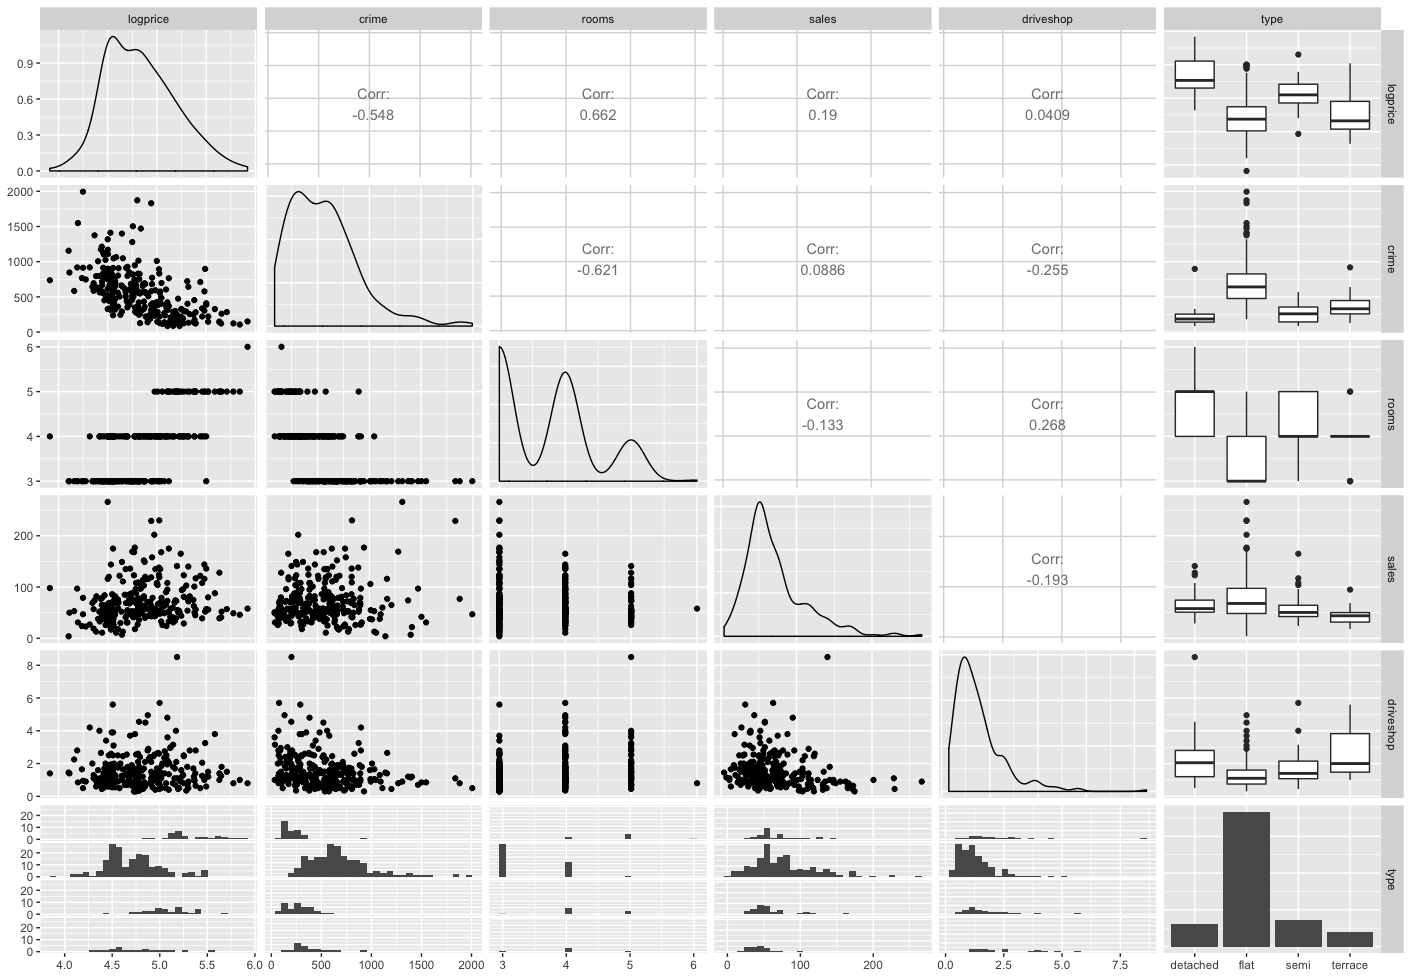
\includegraphics{scatterplot.png}}
\caption{Scatterplot showing the relationships in the data.\label{scatterplot}}
\end{figure} 


\begin{Schunk}
\begin{Sinput}
R> pricedata.sp  <- merge(x=GGHB.IG, y=pricedata, by="IG", all.x=FALSE)
\end{Sinput}
\end{Schunk}
    

Then a spatial map of the \code{price} variable can be overlaid on an OpenStreetMap using the functionality of the \pkg{leaflet} package. However, first the \code{pricedata.sp} object needs to have its coordinate reference system changed to longitude and latitude as this is what the \pkg{leaflet} package requires, which can be done using the following \proglang{R} code.



\begin{Schunk}
\begin{Sinput}
R> library(rgdal)
R> pricedata.sp  <- spTransform(pricedata.sp , 
+                     CRS("+proj=longlat +datum=WGS84 +no_defs"))
\end{Sinput}
\end{Schunk}

Then a map of \code{price} can be drawn using the following code.

\begin{Schunk}
\begin{Sinput}
R> library(leaflet)
R> colours <- colorNumeric(palette = "YlOrRd", domain = pricedata.sp@data$price)
R> map1 <- leaflet(data=pricedata.sp) %>% 
+     addTiles() %>% 
+     addPolygons(fillColor = ~colours(price), color="", weight=1, 
+                 fillOpacity = 0.7) %>%
+     addLegend(pal = colours, values = pricedata.sp@data$price, opacity = 1, 
+                 title="Price") %>%
+     addScaleBar(position="bottomleft")
R> map1
\end{Sinput}
\end{Schunk}


The map is shown in Figure \ref{pricemap} and suggests that Glasgow has a number of property sub-markets, whose prices are not related to those in neighbouring areas. An example of this is the two groups of higher priced regions north of the river Clyde, which are the highly sought after Westerton / Bearsden (northerly cluster) and Dowanhill / Hyndland (central cluster) districts.

\begin{figure}
\centering 
\scalebox{1}{\includegraphics{map1.png}}
\caption{Map showing the average property price in each IG (in thousands).\label{pricemap}}
\end{figure} 


\subsection{Non-spatial modelling}
The natural log of the median property price is treated as the response and assumed to be Gaussian, and an initial covariate only model is built in a frequentist framework using linear models. A model with all the covariates is fitted to the data using the model below.
    
\begin{Schunk}
\begin{Sinput}
R> form <- logprice~crime+rooms+sales+factor(type) + driveshop
R> model <- lm(formula=form, data=pricedata.sp@data)
R> summary(model)
\end{Sinput}
\begin{Soutput}
Call:
lm(formula = form, data = pricedata.sp@data)

Residuals:
    Min      1Q  Median      3Q     Max 
-0.9717 -0.1510 -0.0012  0.1672  0.8346 

Coefficients:
                      Estimate Std. Error t value Pr(>|t|)    
(Intercept)          4.342e+00  1.540e-01  28.203  < 2e-16 ***
crime               -2.248e-04  5.541e-05  -4.057 6.55e-05 ***
rooms                2.119e-01  2.890e-02   7.334 2.79e-12 ***
sales                2.264e-03  3.544e-04   6.388 7.61e-10 ***
factor(type)flat    -2.948e-01  5.988e-02  -4.923 1.51e-06 ***
factor(type)semi    -1.768e-01  5.747e-02  -3.077 0.002312 ** 
factor(type)terrace -3.251e-01  6.921e-02  -4.697 4.26e-06 ***
driveshop           -4.848e-02  1.452e-02  -3.340 0.000961 ***
---
Signif. codes:  0 ‘***’ 0.001 ‘**’ 0.01 ‘*’ 0.05 ‘.’ 0.1 ‘ ’ 1

Residual standard error: 0.2273 on 262 degrees of freedom
Multiple R-squared:  0.6073,	Adjusted R-squared:  0.5968 
F-statistic: 57.88 on 7 and 262 DF,  p-value: < 2.2e-16
\end{Soutput}
\end{Schunk}
    
From the model output above all of the covariates are significantly related to the response at the 5$\%$ level, suggesting they all play an important role in explaining the spatial pattern in median property price. To quantify the presence of spatial autocorrelation in the residuals from this model we compute Moran's I statistic (\citealp{moran1950}) and conduct a permutation test to assess its significance. The permutation test has the null hypothesis of no spatial autocorrelation and an alternative hypothesis of positive spatial autocorrelation, and is conducted using the \code{moran.mc()} function from the \pkg{spdep} package. The test can be implemented using the code below. Lines 2 and 3 turn \code{pricedata.sp} into a neighbourhood (\code{nb}) object and then into a \code{listw} object, which is the required form of the binary spatial adjacency information (based on border sharing) used by the \code{moran.mc()} function.

\begin{Schunk}
\begin{Sinput}
R> library(spdep)
R> W.nb <- poly2nb(pricedata.sp, row.names = rownames(pricedata.sp@data))
R> W.list <- nb2listw(W.nb, style="B")
R> moran.mc(x=residuals(model), listw=W.list, nsim=1000)
\end{Sinput}
\begin{Soutput}
	Monte-Carlo simulation of Moran I

data:  residuals(model) 
weights: W.list  
number of simulations + 1: 1001 

statistic = 0.30141, observed rank = 1001, p-value = 0.000999
alternative hypothesis: greater
\end{Soutput}
\end{Schunk}
    
    
The Moran's I test has  a p-value much less than 0.05, which suggests that the residuals contain substantial positive spatial autocorrelation.


\subsection[Spatial modelling with CARBayes]{Spatial modelling with \pkg{CARBayes}}
The residual spatial autocorrelation can be accounted for by adding a set of random effects to the model, and we apply model (\ref{equation likelihood}) and  (\ref{equation leroux}) to the data as shown below. Note, line 2 creates the binary neighbourhood matrix \code{W} from the \code{W.nb} object.


\begin{CodeInput}
R> library(CARBayes)
R> W <- nb2mat(W.nb, style="B")
R> model.spatial <- S.CARleroux(formula=form, data=pricedata.sp@data, 
+   family="gaussian", W=W, burnin=100000, n.sample=300000, thin=20)
\end{CodeInput}

In the above code the covariate and offset component defined by \code{formula} is the same as for the simple linear model fitted earlier, and the neighbourhood matrix \code{W} is binary and defined by whether or not two areas share a common border. Inference for this model is based on 10,000 MCMC samples, which were obtained following a burn-in period of 100,000 and thinning the remaining 200,000 samples by 20 to reduced their autocorrelation. A summary of the fitted model can be obtained using the following code.

\begin{CodeInput}
R> print(model.spatial)
\end{CodeInput}

\begin{CodeOutput}
#################
#### Model fitted
#################
Likelihood model - Gaussian (identity link function) 
Random effects model - Leroux CAR
Regression equation - logprice ~ ns(crime, 3) + rooms + sales + factor(type) + logdriveshop
Number of missing observations - 0

############
#### Results
############
Posterior quantities and DIC

                     Median    2.5%   97.5% n.sample % accept n.effective Geweke.diag
(Intercept)          4.2423  3.9625  4.5213    10000    100.0     10000.0        -0.4
ns(crime, 3)1       -0.2475 -0.4000 -0.0945    10000    100.0      9398.8        -0.8
ns(crime, 3)2       -0.4081 -0.7055 -0.1105    10000    100.0      9268.4         0.8
ns(crime, 3)3       -0.2021 -0.4052  0.0045    10000    100.0     10000.0         0.4
rooms                0.2205  0.1682  0.2714    10000    100.0     10000.0        -0.3
sales                0.0022  0.0016  0.0029    10000    100.0     10000.0         0.5
factor(type)flat    -0.2474 -0.3660 -0.1279    10000    100.0      9483.0         0.6
factor(type)semi    -0.1616 -0.2606 -0.0598    10000    100.0     10516.5        -0.5
factor(type)terrace -0.2918 -0.4206 -0.1641    10000    100.0     10000.0         0.1
logdriveshop        -0.0055 -0.0621  0.0521    10000    100.0      8321.1         0.5
nu2                  0.0246  0.0146  0.0340    10000    100.0      4364.2         0.3
tau2                 0.0423  0.0196  0.0831    10000    100.0      3626.0        -0.1
rho                  0.9344  0.7499  0.9922    10000     45.5      6323.1         0.2

DIC =  -145.598       p.d =  93.88278       LMPL =  56.89 
\end{CodeOutput}


The Summary is presented in two parts, the first of which describes the model that has been fit. The second summarises the results, and includes the posterior median (\code{Median}) and 95\% credible intervals (\code{2.5\%, 97.5\%}) for selected parameters (not the random effects), the convergence diagnostic proposed by \cite{geweke1992} (\code{Geweke.diag}) as a Z-score, and the effective number of independent samples (\code{n.effective}). Also displayed are the actual number of samples kept from the MCMC run  (\code{n.sample}), as well as the acceptance rate for each parameter (\code{\% accept}). Note, parameters that have an acceptance rate of 100\% have been Gibbs sampled. Finally, the DIC and LMPL  model fit criteria are displayed. In addition to producing the summary above, the model returns a list object with the following components:

\begin{CodeInput}
R> summary(model.spatial)
\end{CodeInput}

\begin{CodeOutput}
Length Class   Mode     
summary.results       91   -none-  numeric  
samples                7   -none-  list     
fitted.values        270   -none-  numeric  
residuals              3   data.frame list   
modelfit               7   -none-  numeric  
accept                 5   -none-  numeric  
localised.structure    0   -none-  NULL     
formula                3   formula call     
model                  2   -none-  character
X                   2700   -none-  numeric  
\end{CodeOutput}



The first element is the summary results table used by the \code{print()} function. The next element is a list containing matrices of the thinned and post burn-in MCMC samples for each set of parameters.  For example, \code{model.spatial$samples$beta} is a matrix containing the MCMC samples for all the regression parameters. The next two elements in the list \code{fitted.values}  and \code{residuals} are vectors of fitted values and residuals from the model, while \code{modelfit} gives a selection of model fit criteria. These criteria include the Deviance Information Criterion (DIC), the log Marginal Predictive Likelihood (LMPL), the Watanabe-Akaike Information Criterion (WAIC), and the log likelihood. For further details about Bayesian modelling and model fit criteria see \cite{gelman2003}. The item \code{accept} contains the acceptance rates for the model, while \code{localised.structure} is \code{NULL} for this model and is used for compatibility with the other functions in the package. Finally, the \code{formula} and \code{model} elements are text strings describing the formula used and the model fit, while \code{X} gives the design matrix corresponding to the \code{formula} object.

\subsection{Inference}
The summary table above gives posterior medians and 95$\%$ credible intervals for a selection of model parameters, but these can be recreated (or similar summarise created for other parameters) using the function

\begin{CodeInput}
R> summarise.samples(model.spatial$samples$beta, quantiles=c(0.5, 0.025, 0.975))
\end{CodeInput}

\begin{CodeOutput}
$quantiles
0.5        0.025       0.975
[1,]  4.241896323  3.962957346  4.51787943
[2,] -0.245877968 -0.396698998 -0.09679782
[3,] -0.401030811 -0.704894560 -0.10461861
[4,] -0.200704600 -0.407327946  0.01018534
[5,]  0.219841199  0.169342794  0.27108763
[6,]  0.002237906  0.001611683  0.00287336
[7,] -0.248767056 -0.368024984 -0.12990882
[8,] -0.162194165 -0.263154252 -0.06109645
[9,] -0.294254065 -0.422182354 -0.16841391
[10,] -0.005002887 -0.061142928  0.04995092

$exceedences
NULL
\end{CodeOutput}


which here has summarised posterior medians and 95$\%$ credible intervals for the covariate effects. However, for the crime variable its relationship is non-linear and summarised by the results for all 3 basis functions \code{ns(crime, 3)1, ns(crime, 3)2, ns(crime, 3)3}. Therefore to summarise the entire non-linear relationship we can use the \code{summarise.lincomb()} function, which allows us to compute the posterior distribution and quantiles of a linear combination of the covariates. This can be achieved and then plotted using the code:


\begin{CodeInput}
R> crime.effect <- summarise.lincomb(model=model.spatial, columns=c(2,3,4), 
+    quantiles=c(0.5, 0.025, 0.975), distribution=FALSE)
R> plot(propertydata.spatial@data$crime, crime.effect$quantiles[ ,1], pch=19, 
+    ylim=c(-0.55,0.05), xlab="Number of crimes", ylab="Effect of crime")
R> points(propertydata.spatial@data$crime, crime.effect$quantiles[ ,2], pch=19, 
+   col="red")
R> points(propertydata.spatial@data$crime, crime.effect$quantiles[ ,3], pch=19, 
+   col="red")
\end{CodeInput}


\begin{figure}
\centering 
\scalebox{1}{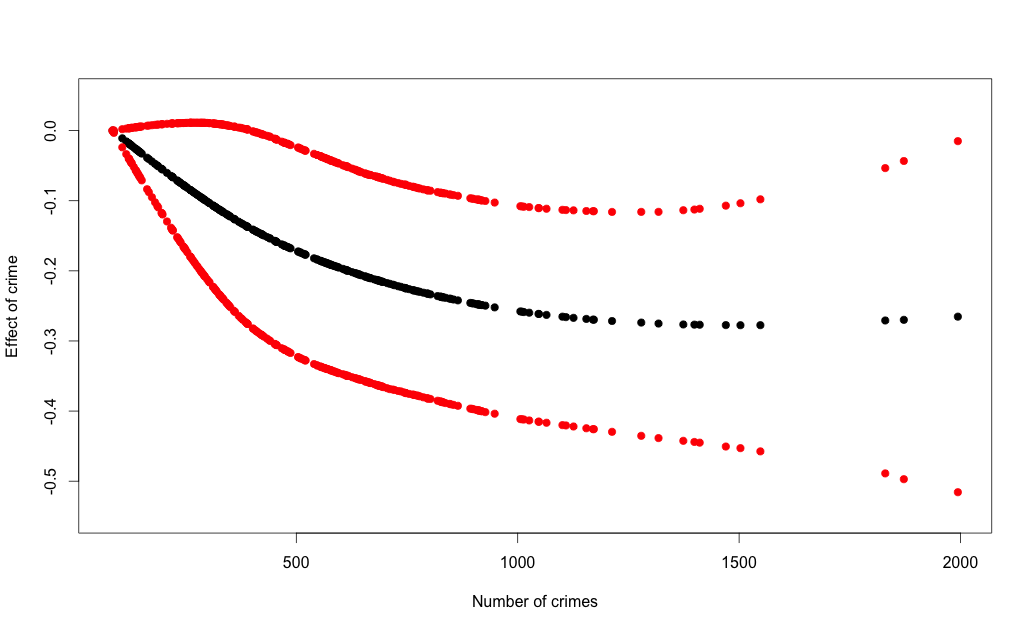
\includegraphics{crimeplot.png}}
\caption{Plot showing the estimated non-linear relationship between crime rate and log-price.\label{crimeplot}}
\end{figure} 

The first line creates the crime effect, while the remaining lines plot the graph which is shown in Figure \ref{crimeplot} and shows a decreasing relationship as crime rate increases as expected.


\section{Example 3 - identifying high-risk disease clusters}
The third example illustrates the utility of the localised spatial autocorrelation model proposed by \cite{lee2012}, which can identify boundaries that represent step changes in the (random effects) response surface between geographically adjacent areal units. The aim of this analysis is to identify boundaries in the risk surface of respiratory disease in Greater Glasgow, Scotland, in 2010, so that the spatial extent of high-risk clusters can be identified. The identification of boundaries in spatial data is affectionately known as \emph{Wombling}, after the seminal paper by \cite{womble1951}. 


\subsection{Data and exploratory analysis}
The data again relate to the Greater Glasgow and Clyde health board, and are also freely available to download from  Scottish Statistics (\emph{http://statistics.gov.scot}). However, the river Clyde partitions the study region into a northern and a southern sub-region, and no areal units on opposite banks of the river border each other. This means that boundaries could not be identified across the river, and therefore here we only consider those areal units that are on the northern side of the study region. This leaves 134 areal units in the new smaller study region, and data on respiratory disease for this region are included with the \pkg{CARBayesdata} package and can be loaded with the command:


\begin{Schunk}
\begin{Sinput}
R> library(CARBayesdata)
R> library(sp)
R> data(GGHB.IG)
R> data(respiratorydata)
\end{Sinput}
\end{Schunk}

The \code{GGHB.IG} \code{spatialPolygonsDataFrame} object can then be subset to just include IGs in the \code{respiratorydata} data.frame using the following code.

\begin{Schunk}
\begin{Sinput}
R> respiratorydata.spatial <- merge(x=GGHB.IG, y=respiratorydata, by="IG", all.x=FALSE)
\end{Sinput}
\end{Schunk}

The first 6 rows of the data can be viewed using the code below.


\begin{Schunk}
\begin{Sinput}
R> head(respiratorydata.spatial@data)
\end{Sinput}
\begin{Soutput}
         IG                         name  easting northing observed  expected
1 S02000260                   Auchinairn 261624.5 669657.4      107 106.45661
2 S02000261                Woodhill East 262927.1 670027.8       23  50.97354
3 S02000262                Woodhill West 262142.9 670428.0       53 104.49236
4 S02000263               Westerton East 254570.5 670593.8       40  90.35747
5 S02000264 Bishopbriggs West and Cadder 261248.4 670928.0       60 140.16546
6 S02000265               Westerton West 253764.4 670982.6       25  63.93549
  incomedep       SMR
1        22 1.0051044
2         7 0.4512145
3         6 0.5072141
4         5 0.4426861
5         7 0.4280655
6         6 0.3910191
\end{Soutput}
\end{Schunk}

In addition to the unique identifier IG codes (\code{IG}), the name of each IG (\code{name}), and the geographical coordinates of each area's centroid (\code{easting, northing}), the data contain 4 variables.  \code{observed} is the  number of hospital admissions in 2010 in each IG due to respiratory disease (International Classification of Disease tenth revision codes J00-J99). These observed numbers will depend on the size and demographic structure of the populations living in each IG, and these factors need to be adjusted for before estimating disease risk. This is typically achieved  by computing the expected numbers of hospital admissions in each IG based on this demographic information, using indirect standardisation. These expected numbers are stored in the \code{expected} column, and the simplest measure of disease risk is the Standardised Morbidity Ratio (SMR), which is the ratio of the observed to the expected numbers of hospital admissions and is stored in the \code{SMR} column. Finally, the percentage of people defined to be income deprived (in receipt of means tested benefits) is stored in the \code{incomedep} column. A map showing the SMR is displayed in Figure \ref{smrmap}, and is created using the code below, where in common with the previous example the coordinate reference system is changed to longitude and latitude.



\begin{Schunk}
\begin{Sinput}
R> respiratorydata.spatial <- spTransform(respiratorydata.spatial, 
+                                     CRS("+proj=longlat +datum=WGS84 +no_defs"))
R> library(leaflet)
R> colours <- colorNumeric(palette = "BuPu", domain = respiratorydata.spatial@data$SMR)
R> map2 <- leaflet(data=respiratorydata.spatial) %>% 
+     addTiles() %>% 
+     addPolygons(fillColor = ~colours(SMR), color="red", weight=1, 
+                 fillOpacity = 0.7) %>%
+     addLegend(pal = colours, values = respiratorydata.spatial@data$SMR, opacity = 1, 
+                 title="SMR") %>%
+     addScaleBar(position="bottomleft")
R> map2
\end{Sinput}
\end{Schunk}
    
    
\begin{figure}
\centering 
\scalebox{1}{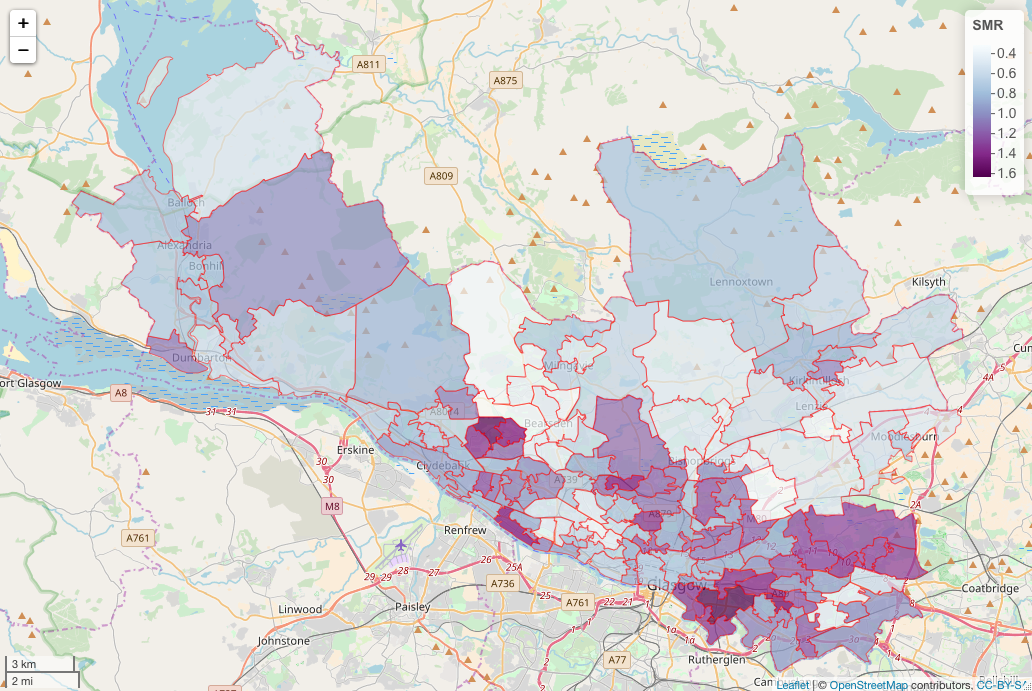
\includegraphics{map2.png}}
\caption{Map displaying the SMR for each area.\label{smrmap}}
\end{figure} 


Values of the SMR above one relate to areas exhibiting above average risks, while values below one correspond to below average risks. For example, an SMR of 1.2 corresponds to a 20\% increased risk relative to the expected numbers of respiratory disease cases. The figure shows evidence of localised spatial structure, with numerous different locations where high and low risk areas border each other. This in turn suggests that boundaries are likely to be present, and their identification is the goal of this analysis. The method proposed by \cite{lee2012} identifies these boundaries using dissimilarity metrics, which are non-negative measures of the dissimilarity between all pairs of adjacent areas. In this example we use the absolute difference in the percentage of people in each IG who are defined to be income deprived (\code{incomedep}), because it is well known that socio-economic deprivation plays a large role in determining people's health. However, before fitting the model the spatial neighbourhood matrix $\mathbf{W}$ based on sharing a common border is computed using the following code.



\begin{Schunk}
\begin{Sinput}
R> W.nb <- poly2nb(respiratorydata.spatial, row.names = 
+                 rownames(respiratorydata.spatial@data))
R> W <- nb2mat(W.nb, style="B")
\end{Sinput}
\end{Schunk}



\subsection[Spatial modelling with CARBayes]{Spatial modelling with \pkg{CARBayes}}
Let the  observed and expected numbers of hospital admissions be denoted by $\mathbf{Y}=(Y_{1},\ldots,Y_{K})$ and $\mathbf{E}=(E_{1},\ldots,E_{K})$ respectively. Then as the observed numbers of hospital admissions are counts, a Poisson likelihood model given by $Y_{k}\sim\mbox{Poisson}(E_{{k}}R_{k})$ is appropriate, where $R_{k}$ represents disease risk in areal unit $\mathcal{S}_{k}$. A log-linear model is specified for $R_{k}$, that is, $\ln(R_{k})=\beta_{0}+\phi_{k}$, and for a general review of disease mapping see \cite{wakefield2007}. We note that in fitting this model in \pkg{CARBayes}, the offset is specified on the linear predictor scale rather than the expected value scale, so in this analysis the offset is $\log(\mathbf{E})$ rather than $\mathbf{E}$. The dissimilarity metric used here is the absolute difference in the level of income deprivation between each pair of areal units, which can be created from the  vector of area level income deprivation scores using the following code.

\begin{Schunk}
\begin{Sinput}
R> income <- respiratorydata.spatial@data$incomedep
R> Z.incomedep <- as.matrix(dist(income, diag=TRUE, upper=TRUE)) 
\end{Sinput}
\end{Schunk}

The first line pulls out the income deprivation covariate while the second line computes the $K\times K$ matrix of absolute differences in income deprivation levels between each pair of areal units, that is \code{Z.incomedep}$_{kj}$ = |\code{income}$_{k}$ - \code{income}$_{j}$|. The function to implement the localised CAR model is called \code{S.CARdissimilarity()}, and it takes the same arguments as the other CAR models except that it additionally requires the dissimilarity metrics. These are required in the form of a list of $K\times K$ matrices, and for this example we only have a single dissimilarity metric. Additionally, we add the argument \code{W.binary=TRUE}, so that the estimated elements in $\mathbf{W}$ are ones or zeros (corresponding to (\ref{equation binary neighbourhood})), the latter corresponding to boundaries. The model is run using the following code.




\begin{CodeInput}
R> formula <- observed ~ offset(log(expected))
R> model.dissimilarity <- S.CARdissimilarity(formula=formula, 
+    data=respiratorydata.spatial@data, family="poisson", W=W, 
+    Z=list(Z.incomedep=Z.incomedep), W.binary=TRUE, burnin=100000, 
+    n.sample=300000, thin=20)
R> print(model.dissimilarity)
\end{CodeInput}


\begin{CodeOutput}
#################
#### Model fitted
#################
Likelihood model - Poisson (log link function) 
Random effects model - Binary dissimilarity CAR 
Dissimilarity metrics -  Z.incomedep 
Regression equation - observed ~ offset(log(expected))
Number of missing observations - 0

############
#### Results
############
Posterior quantities and DIC

             Median    2.5%   97.5% n.sample % accept n.effective Geweke.diag alpha.min
(Intercept) -0.2197 -0.2414 -0.1987    10000     35.2     10000.0        -0.5        NA
tau2         0.1373  0.0980  0.1927    10000    100.0      9089.8        -0.5        NA
Z.incomedep  0.0500  0.0464  0.0513    10000     45.4     10000.0         0.3    0.0139

DIC =  1070.334       p.d =  105.4371       LMPL =  -615.38 

The number of stepchanges identified in the random effect surface
     no stepchange stepchange
[1,]           261         99
\end{CodeOutput}

The first line of the above code specifies the formula with an offset (the natural log of the expected numbers of cases) but no covariates, the latter being required so that boundaries identified in the random effects surface can also be interpreted as boundaries in the risk surface (that is boundaries in $\mathbf{R}=(R_{1},\ldots,R_{n})$). The above model bases inference on 10,000 post burn-in and thinned MCMC samples. When the model has been fit the \code{print()} function produces the summary output above, which is similar to that produced for the property price data in the previous example. The main difference between this and the corresponding output from the property price analysis is the addition of a column in the parameter summary table headed \code{alpha.min}. This column only applies to the dissimilarity metrics, which is why it is \code{NA} for the remaining parameters. The value of \code{alpha.min} is the threshold value for the regression parameter $\alpha$, below which the dissimilarity metric has no effect in identifying boundaries in the response (random effects) surface. A brief description is given in Section 2.1, while full details are given in \cite{lee2012}. For these data the posterior median and 95$\%$ credible interval lie completely above this threshold, suggesting that the income deprivation dissimilarity metric has identified a number of boundaries.

\hspace{1cm}The number and locations of these boundaries are summarised in the element of the output list called \code{model.dissimilarity$localised.structure$W.posterior}, which is a $K\times K$ symmetric matrix containing the posterior median for the set $\{w_{kj}|k\sim j\}$. Values equal to zero represent a boundary, values equal to one correspond to no boundary, while \code{NA} values correspond to non-adjacent areas. The locations of these boundaries can be overlaid on a map of the estimated disease risk (that is the posterior median of $\mathbf{R}$). This is done in two steps, the first being the creation of a \code{SpatialPoints} object using the following code. 

\begin{CodeInput}
R> border.locations <- model.dissimilarity$localised.structure$W.posterior
R> respiratorydata.spatial@data$risk <- model.dissimilarity$fitted.values / 
+   respiratorydata.spatial@data$expected
R> boundary.final <- highlight.borders(border.locations=border.locations, 
+   spdata=respiratorydata.spatial)
\end{CodeInput}

The first line saves the matrix of border locations, while the second adds the estimated risk values to the \code{respiratorydata.spatial} object. The next line identifies the boundary points (using the \pkg{CARBayes} function \code{highlight.borders()}) and formats them to enable plotting. Then plotting can be done using the code below, and the result is presented in Figure \ref{figure_boundary}.


\begin{CodeInput}
colours <- colorNumeric(palette = "BuPu", domain = respiratorydata.spatial@data$risk)
map3 <- leaflet(data=respiratorydata.spatial) %>% 
    addTiles() %>% 
    addPolygons(fillColor = ~colours(risk), color="red", weight=1, 
                fillOpacity = 0.7) %>%
    addLegend(pal = colours, values = respiratorydata.spatial@data$risk, opacity = 1, 
                title="Risk") %>%
    addCircles(lng = ~boundary.final$X, lat = ~boundary.final$Y, weight = 1, 
                radius = 2) %>%
    addScaleBar(position="bottomleft")
map3
\end{CodeInput}

\begin{figure}
\begin{center}
\scalebox{1.2}{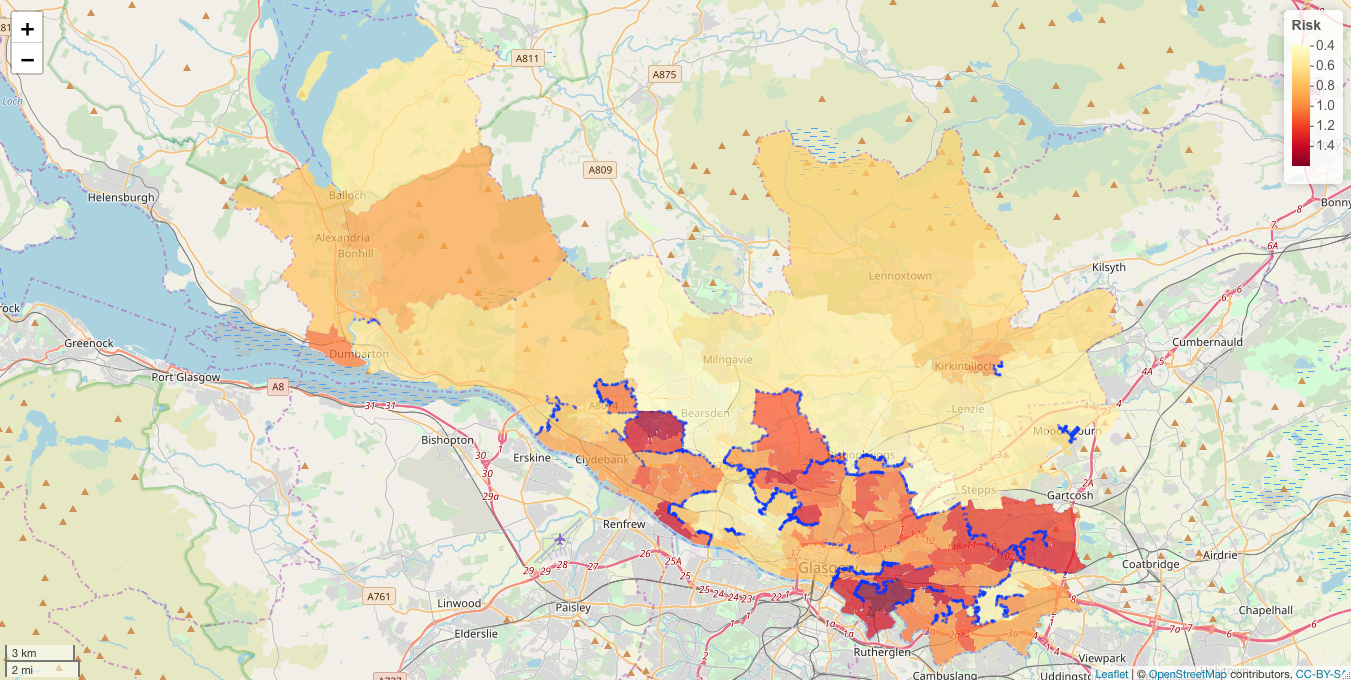
\includegraphics{map3.png}}
\end{center}
\vspace{-1cm}\caption{Map displaying estimated risk and locations of the boundaries for the northern part of Greater Glasgow.}\label{figure_boundary}
\end{figure}


The figure shows the fitted risk surface and the locations of the boundaries (denoted by blue circles).  The model has identified 99 boundaries in the risk surface. The majority of these visually seem to correspond to sizeable changes in the risk surface, suggesting that the model has the power to distinguish between boundaries and non-boundaries. The notable boundaries are the demarcation between the low risk (shaded green) city centre / west end of Glasgow in the middle of the region and the deprived neighbouring areas on both sides, which include Easterhouse / Parkhead in the east and Knightswood / Drumchapel in the west. The other interesting feature of this map is that the boundaries are not closed, suggesting that the spatial pattern in risk is more complex than being partitioned into groups of non-overlapping areas of similar risk.


\section{Discussion}
This vignette has illustrated the \proglang{R} package \pkg{CARBayes}, which can fit a number of commonly used  conditional autoregressive models to spatial areal unit data, as well as the localised spatial smoothing models proposed by \cite{lee2012} and \cite{lee2015}. The response data can be binomial, Gaussian, multinomial, Poisson or ZIP, with link functions logit, identity, logit, natural log and (natural log / logit) respectively. The availability of areal unit data has grown dramatically in recent times, due to the launch of freely available on-line databases. This increased availability of spatial data has fuelled a growth of modelling in this area, leading to the need for user friendly software such as \pkg{CARBayes} for use by both statisticians and non-statisticians alike. Finally, this software now has a sister spatio-temporal modelling package called \pkg{CARBayesST}, which can fit a range of spatio-temporal areal unit models based on CAR priors. These models include similar models to those proposed by \cite{bernardinelli1995} and \cite{knorrheld2000b}, as well as other alternatives.

\section*{Acknowledgements}
The data and shapefiles used in sections 5 and 6 of this vignette were provided by the Scottish Government.


\bibliography{jss996}
\end{document}


